% !TeX program = lualatex
\documentclass[a4paper,12pt,twoside]{article}
\usepackage{hot_report}
\usepackage[utf8]{inputenc}

\title{Displaced Persons Head Counts}
\author{Sara Amadi, Asha Mustapher, Johanes Petro, Barnabas Caro, Ivan Gayton }
\date{July 2019}

\begin{document}

\maketitle


\renewcommand{\baselinestretch}{1.5}\normalsize %the number controls the spacing between ToC lines
\tableofcontents
\renewcommand{\baselinestretch}{1.0}\normalsize

\newpage

\section{Executive Summary}
\begin{multicols}{2}
We interviewed ten teams---four MSF and six from other agencies---working in contexts of displacement in East Africa, often in closed (camp-like) settings as well as a few open settings. In most cases they considered a population estimate important to their work, though the perceived utility and use-case varied; the most compelling use-cases being for resource allocation (food, NFIs, etc) and public health (vaccination and health coverage). 

Most teams reported at least some dissatisfaction with existing "traditional" methods of conducting population estimates or head counts. Most reported bias in the available sources; people, agencies, and governments often have incentives to manipulate these numbers. 

Attitudes toward technological methods such as drones and mobile device-based surveys varied from considering them out of the question to regarding them as potential avenues to escape the usual pitfalls. In some cases teams within the same country perceived the risks quite differently, suggesting that the risks are not actually well-known or consistently analysed. 

We propose a typology of contexts and needs to determine where technological head count methods may be useful (helping create positive impact for displaced people) and practicable (safe, ethically permissible, and achievable). Furthermore we propose some methods whereby these methods can be selected and undertaken.

A great many options are possible, some low-cost, low-risk, and relatively simple, others more disruptive, high-tech, and risky. In many cases, simple, non-risky, low-tech options are preferable. Paper surveys, sketch maps, discussions with local staff and patients, and community dialogue, the bread and butter of humanitarian medical intervention, remain fundamentally sound tools.

However, there is value in expanding the MSF palette with riskier, more disruptive methods. These are emphatically not appropriate for all contexts, and it is not yet clear where and when they are safe and effective. Therefore we suggest attempting to choose one or more sites where a simple pilot can be conducted using one or more of the methods discussed here, including aerial imagery and community-driven mobile device-based surveying\footnote{MSF and other agencies already have substantial expertise and capacity to implement mobile device-based surveys using OpenDataKit, KoBo Toolbox, MWater, CommCare, and other platforms. However, doing so primarily using relatively uneducated and untrained people from within the displaced community itself seems to be rare.}. We provide some guidance on practical implementation of these methods, including cost estimates and a risk assessment framework.

\end{multicols}

\newpage
\section{Introduction}
\begin{multicols}{2}
MSF often needs to know the number of displaced people in a camp, settlement, Protection of Civilians area, or other context. Population numbers are useful to prioritize contexts where there aren't enough resources to respond to all of the calls for help. They can facilitate rational HR and supply planning, and inform advocacy in cases where other actors are not taking their responsibilities to meet the needs of the population (as with inadequate food distributions). 

"Head counts" are difficult to perform accurately, safely, and ethically. They can be fraught with economic incentives---people and agencies often attempt to exaggerate numbers to attract funding---and political sensitivities. Governments, in an attempt to deny the existence of problems in their territory, may attempt to pressure agencies to under-count displaced persons (or to exaggerate them to attract funding or international attention and sympathy). Some methods of counting people are coercive and dangerous---for example people may be forced into barbed-wire enclosures for counting purposes---and MSF will not wish to participate in such activities despite wishing to have accurate population figures. 

We have looked at a number of settings where head counts are needed, and asked
those intervening what population information they need, what they actually have, the shortcomings of that information, and how they currently address it. We are now proposing several potential methods to improve upon the status quo. These are informed by the information we have gathered here as well as our work with the Missing Maps project.

Our recommendations include relatively novel techniques such as drone surveys and mobile data collection using unskilled community members. These are not intended to be prescriptive or exhaustive, but rather to point the way toward several possible pilot projects. Additionally, we discuss the many ethical, practical, and security-related limitations of these methods, and propose a basic framework to assess the appropriateness of various head count methods.

\end{multicols}

\section{Context and Need Typology}
\begin{multicols}{2}
Before deciding to do a head count---and choosing a method---first assess what population data is available, why you need the population figures, and what exact information you need. 

For example, in the case of a rapid displacement in the range of hundreds of thousands of people arriving in an unprepared camp site, it's likely that the immediate need will be a very rough count---just sufficient to order a sensible number of plastic sheets, jerry cans, vaccine doses, and food. In such cases, political and access constraints may be such that a rough count is all that is feasible, and disruptive technological methods are often not accepted by those in power (or by the---often traumatized---population).

In other cases, for example, a long-established camp setting, improving medical quality and ensuring the most vulnerable receive care may require detailed information from each household or a considerable sample size---number of children, vulnerable members, pregnant women, and so forth. The choice of tools should follow from the needs.

\end{multicols}

\newpage
At the risk of oversimplifying, we have chosen several broad categories of need for population counts:
\begin{itemize}
    \item Rapid household count (usually counting tents or structures)
    \item Rapid household survey (counting the residents of each structure or a sample subset thereof)
    \item Detailed household survey (enumerating the residents of structures, including demographic information)
\end{itemize}

Any of these may furthermore be needed on a frequent basis. Monitoring changes in population can be important; for example people in a Protection of Civilians (PoC) zone may fluctuate dramatically due to contextual factors (entering when violence levels are high, and leaving either when violence is lower or when other factors such as harvest seasons compel people to risk going back to their homes). For this reason, all of the above categories may be needed on different time-scales; in some cases a single baseline may be all that is needed, and in others a monthly or even weekly estimate may help teams to understand the needs of their beneficiaries and the context outside of the displacement settlement (i.e. extrapolating violence levels or food availability from camp population). 

\subsection{Rapid Household Count}
 This does not enumerate all residents, but only counts the households, typically by using tents or other structures as a proxy for the number of people. We usually do not visit each structure, but simply estimate the number of structures and multiply by an expected number of people per structure.

\noindent
\textbf{Examples of use-cases:}

\begin{itemize}
  \item Recent displacement
  \item To estimate the resources needed for blanket distributions
  \item To compare and prioritize needs between several potential interventions
\end{itemize}

\noindent
\textbf{Possible Methods:}

\begin{itemize}
  \item From above
  \begin{itemize}
    \item Satellite
    \item Aircraft (plane or helicopter)
    \item Drone (fixed-wing or multicopter)
    \item Balloon or kite
  \end{itemize}
\end{itemize}

\begin{itemize}
  \item From the ground
  \begin{itemize}
    \item GPS survey to get total area, multiply by structure density and persons/structure
    \item Count rows and columns, multiply for structure count
  \end{itemize}
\end{itemize}

\begin{itemize}
    \item Remote data aggregation
    \begin{itemize}
        \item Crowdsourcing; self-census using SMS or social media/messaging
        \item Artificial Intelligence/Machine Learning based on social media, weather, news, or other parameters
        \item Data from telecommunications (calling patterns or mobile handset registration with different towers)
        \item Profiling populations pre-displacement (birth data etc)
    \end{itemize}
\end{itemize}

\noindent
\textbf{Completion time: 1-3 days}

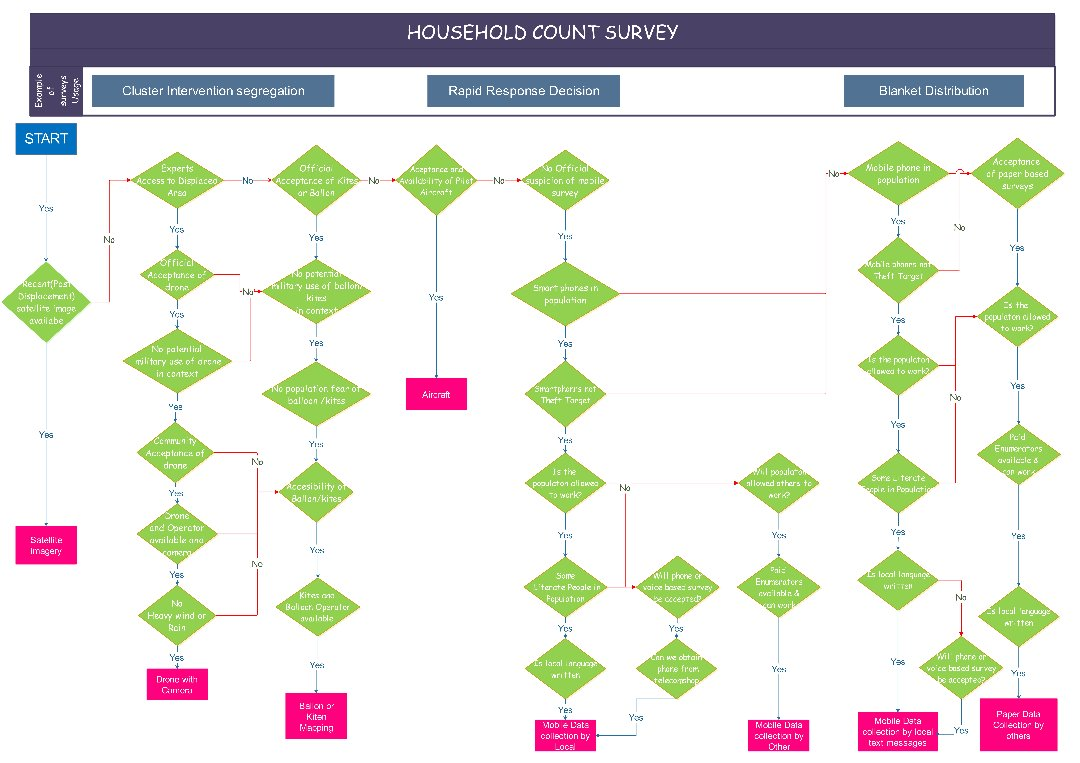
\includegraphics[width=1\textwidth]{images/Household_Count.jpeg}

\newpage
\subsection{Rapid Household Survey}
This method provides more detail on the demographics of the population, typically at least the number of men, women, and children. Here we visit each structure and speak to the residents, but gather only basic information (number of people disaggregated by age and sex) for each household. This very simple data can usually be collected quickly with relatively low-skilled enumerators.

\noindent
\textbf{Examples of use-cases:}

\begin{itemize}
    \item To conduct a basic needs assessment for a given population (i.e. ordering supplies)
    \item To determine the extent and distribution of primary health care needed for patients
\end{itemize}

\noindent
\textbf{Possible Methods:}
\begin{itemize}
    \item Mobile Data Collection
    \item Paper-based surveys
    \item Aggregate medical records and "denominator tool" calculations
    \item Spatial sampling with a subset of households surveyed
\end{itemize}

\noindent
\textbf{Completion time:} 1-2 weeks

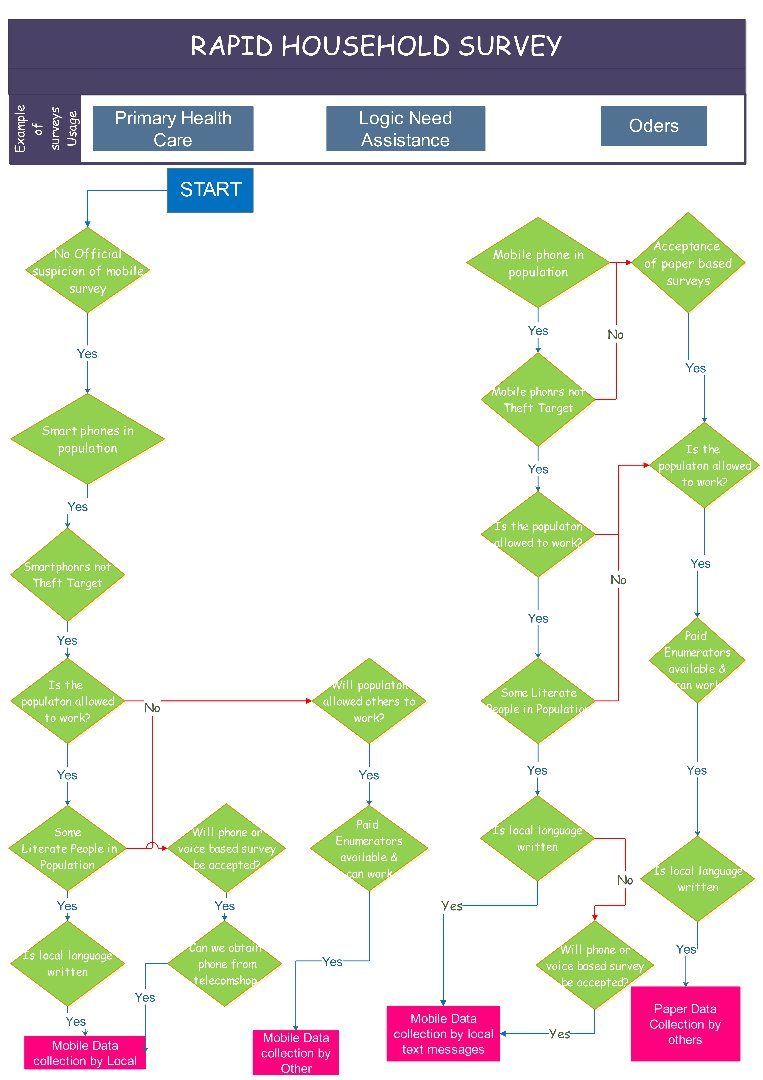
\includegraphics[width=0.9\textwidth]{images/Rapid_Household_Survey.jpeg}

\subsection{Detailed Household Survey}
Sometimes you need to understand the demographics, vulnerability, and specific characteristics of people within each household. In this case you will conduct an extensive survey at each household (though this may be not be every household---it may be a subset chosen as a sample from which to extrapolate the characteristics of the whole population). 



\noindent
\textbf{Examples of use-cases:}
\begin{itemize}
    \item Established camp where we feel that some people do not have access to care and may not be presenting in clinics
    \item Setting where a subset of the population is unusually vulnerable, such as malnourished children, HIV/TB-positive people, etc
    \item Setting with seemingly unexplained mortality
    \item Setting where MSF needs to advocate on behalf of a specific segment of the population (i.e. women lacking access to safe firewood collection) and wishes to have concrete numbers with which to call for others to take their responsibilities
\end{itemize}

\noindent
\textbf{Possible Methods:}
\begin{itemize}
    \item Mobile Data Collection
    \item Paper-based surveys
    \item Spatial sampling with a subset of households surveyed
    \item Integration of mobile data collection into Community Health Worker and outreach practice
\end{itemize}

\noindent
\textbf{Completion time: 1 month to ongoing}

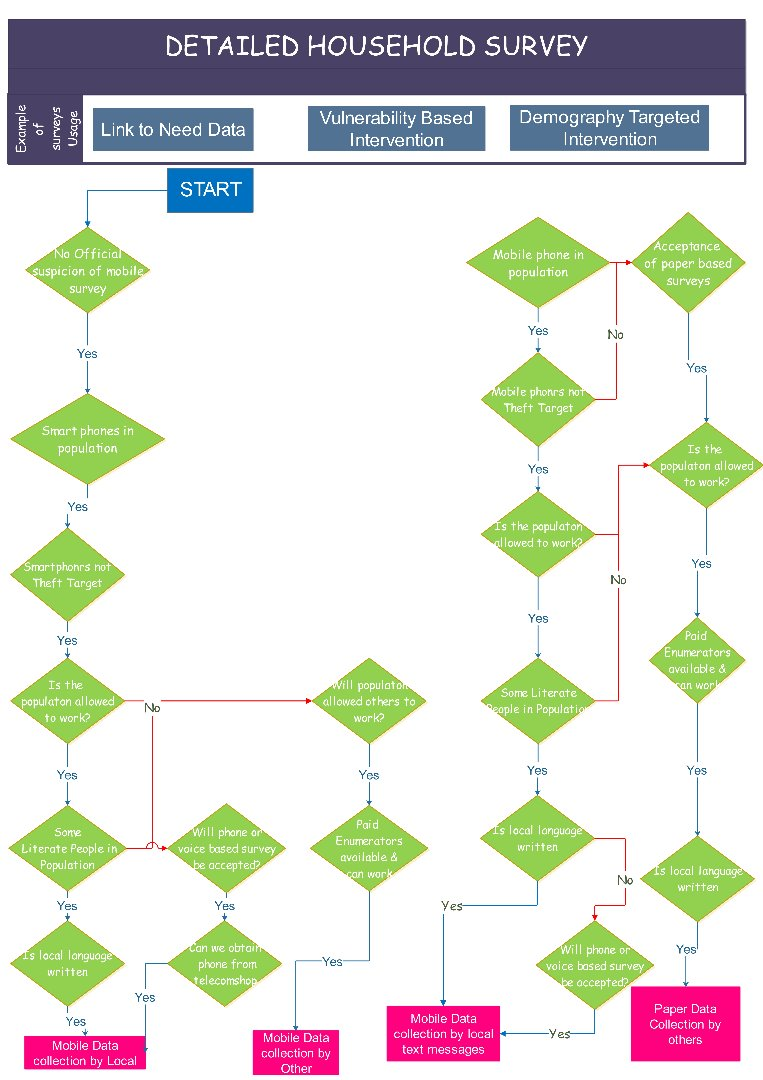
\includegraphics[width=0.9\textwidth]{images/Detailed_Household_Survey.jpeg}

\section{Tool Options}
Here we examine several families of tools for conducting population estimates. 

\subsection{Comparison of Tools}

\begin{tabular}{c|c}
     &  \\
     & 
\end{tabular}

\subsection{Aerial Mapping}
In displacement settings where new shelters are constructed, the shelters themselves can serve as a proxy for population numbers. Shelters can be seen from above, whether by satellite, aircraft, drone, or other method providing an "eye in the sky." 

This is risky; displaced people and those responsible for responding to their needs are more than capable of anticipating such an effort and constructing visible structures to fool the viewer into thinking there are more people present (a team we interviewed from the Danish Refugee Council cited a case in Kenya where refugees became aware that new satellite imagery was being collected in the area and began building additional "fake" structures).

In settings where displaced people are hosted within an existing population, shelter counts are usually ineffective; you can't really tell from above whether a house contains a single family or is hosting several displaced families at a much higher density\footnote{Technologies such as infrared sensing are capable in theory of determining the number of people within a structure---an infrared camera detects body heat and can to some extent see through a roof. However, these methods are quite expensive and delicate. Even more problematic, such methods and equipment are primarily used for military purposes, and therefore are problematic, both perceptually and in the potential for abuse of the information.}. 

However, in settings of recent displacement where the field team is relatively confident that visible shelters do represent a reasonably proxy for population and needs, aerial counts may be the single most effective rapid population estimation tool currently available. 

\subsubsection{Drones}
\textbf{N.B.} This section discusses the technical aspects only of drone use for displaced population estimation. It presupposes that the ethical, perceptual, and security issues have already been addressed. 

Unmanned Aerial Vehicles (UAVs) or drones come in two basic flavors: fixed-wing and multirotor. 

\begin{figure}[H]
\begin{subfigure}{0.5\textwidth}
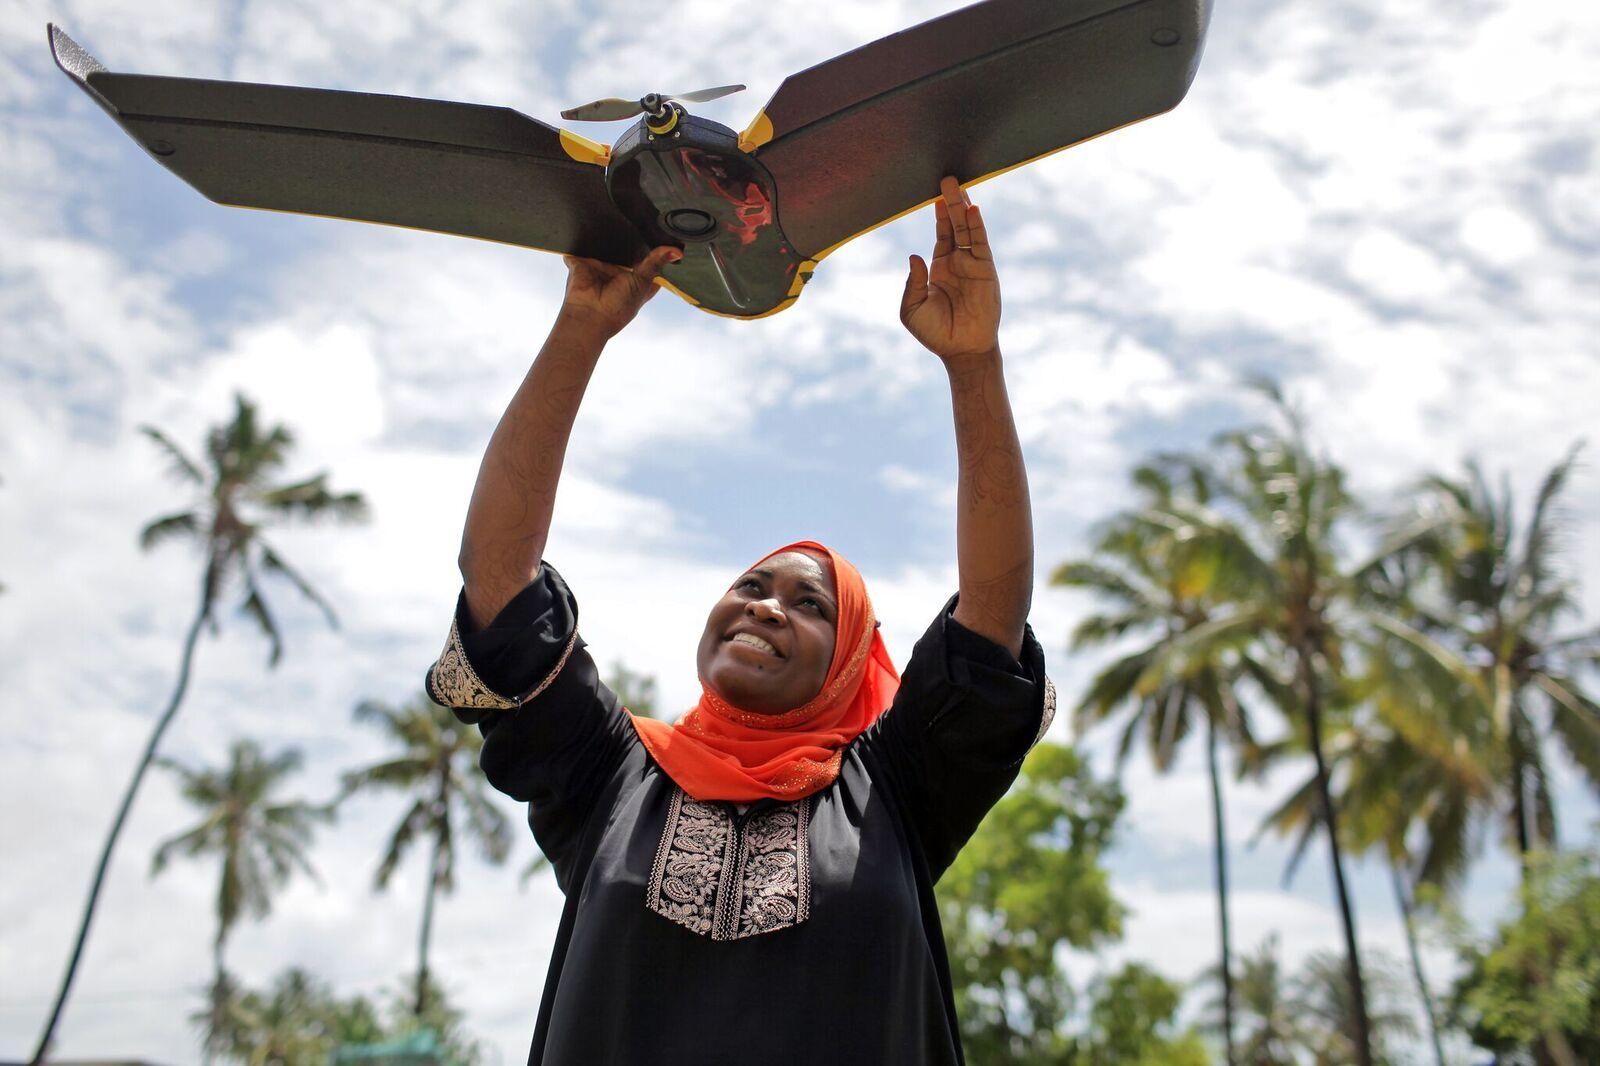
\includegraphics[width=0.9\linewidth, height=5cm]{images/Zanzibar_ebee.jpg} 
\caption{Fixed-wing drone: Sensefly Ebee}
\label{fig:subim1}
\end{subfigure}
\begin{subfigure}{0.5\textwidth}
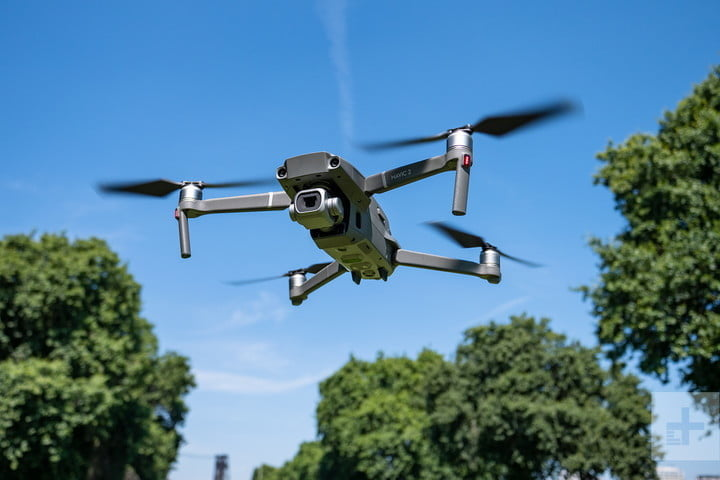
\includegraphics[width=0.9\linewidth, height=5cm]{images/dji-mavic-2-pro.jpg}
\caption{Multirotor drone: DJI Mavic Pro 2}
\label{fig:subim2}
\end{subfigure}
\caption{Two types of Unmanned Aerial Vehicles (UAVs or drones)}
\label{fig:image2}
\end{figure}


Multirotor drones are inexpensive\footnote{A DJI Mavic Pro 2, which is capable of autonomous flight for mapping, costs about \$1600 and can be carried as hand luggage on a commercial airline flight.}, small, and quite safe. They do not require enormous expertise or resources to operate, and as they are increasingly common consumer items (frequently used for wedding photography, even in low-income and unstable countries\footnote{In Pakistan, which many people expect to be very sensitive to drones due to military uses, drone wedding photography using small multirotors is enormously popular.}) Due to the intense energy demand of hovering in mid-air, multirotor drones have much shorter flight times than fixed-wing drones, and therefore can map much less area per flight.

Fixed-wing surveying drones such as the Sensefly Ebee are much more expensive than consumer multirotors\footnote{the Ebee costs around \$15,000 to purchase, but also requires licenses for proprietary software to unlock many of its functions; this can add substantial expense to operations)}. Because they make use of a wing to stay aloft, they are much more energy-efficient than multirotors and can capture imagery for a greater area per flight.

A single Ebee flight can map on the order of 1km\textsuperscript{2} with an image resolution of 7cm/pixel. In a day, an experienced operator can make up to ten flights (though six is more usual). For the sake of comparison, Dadaab Refugee Camp in Kenya has an area of 2.4km\textsuperscript{2}; it could easily be covered by high-resolution imagery in a single day's operation of an Ebee or similar drone. Nearby Dagahaley camp, covering approximately 9km\textsuperscript{2}, could be covered in one to two days.

\begin{figure}[H]
    \centering
    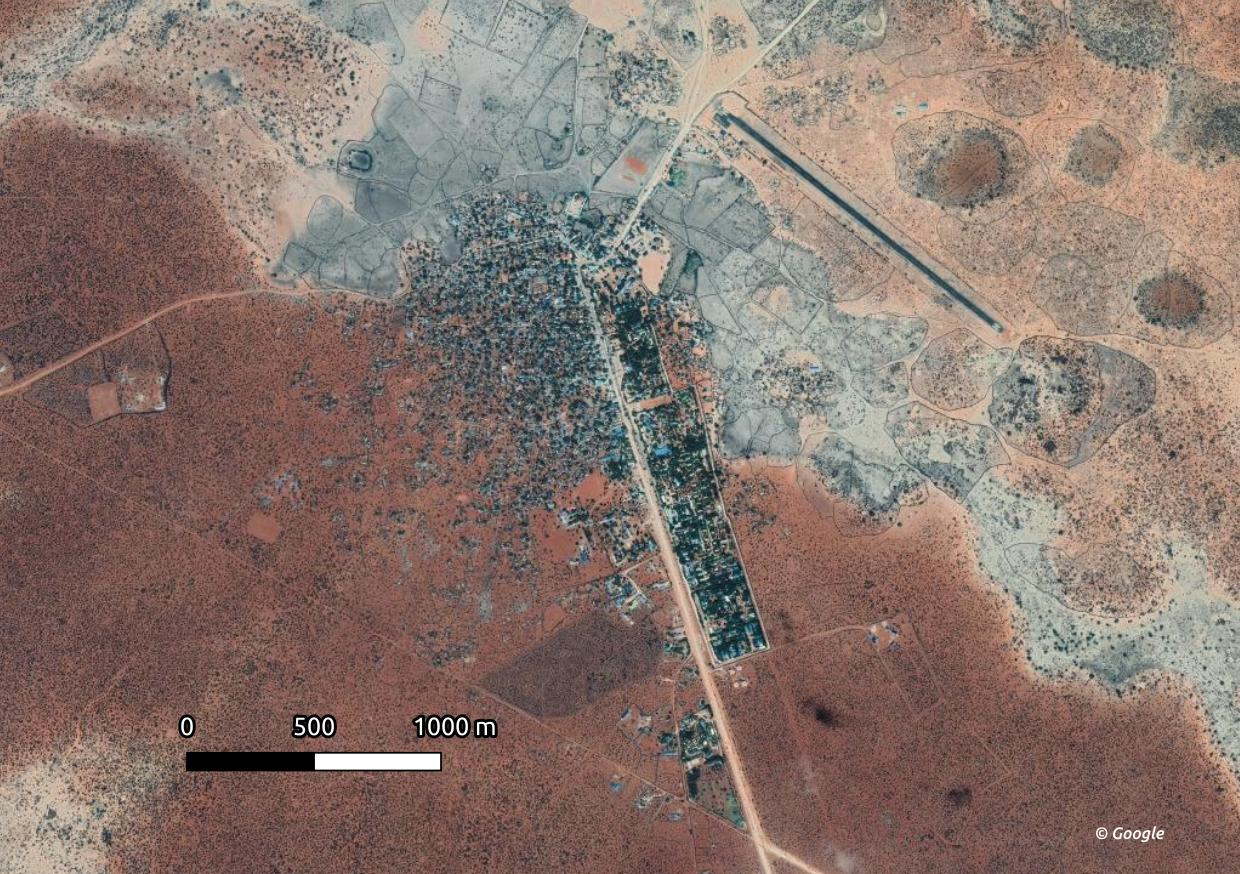
\includegraphics[width=0.6\textwidth]{images/dadaab.jpeg}
    \caption{Dadaab Refugee Camp in Eastern Kenya}
    \label{fig:Dadaab Refugee Camp}
\end{figure}

At the time of writing (mid-2019) the most efficient method of gathering aerial imagery on the scale of a refugee camp (several square kilometers) in sub-Saharan Africa is probably the use of an Ebee or similar fixed-wing drone. 

As an example of a deployment, a team based in Tanzania with an Ebee\footnote{This information comes from an actual drone operator who often works with the authors of this report: uhurulabs.com. Uhurulabs is, of course, not the only option and we recommend that MSF choose providers based on an objective procurement process (thus ends the "not saying you have to hire our friends" disclaimer), but we are grateful for Uhurulabs' willingness to share details of their operating costs.} can deploy to anywhere within East Africa within 48 hours\footnote{A team's ability to actually enter the country depends on specific regulations and immigration procedures, but in most cases this can be managed, particularly if the activities are part of a mission that already has a reasonable relationship with local authorities; typically a Letter of Invitation from an NGO---or better yet the Ministry of Health---is sufficient to clear Immigration with an Ebee.} The cost of such a team with their equipment (two people and an Ebee with ancillary gear) is approximately \$1,000 per flying day, exclusive of travel airfare (but including all other expenses such as prep time and image processing). 

At least one day is required to inform and sensitize local officials and the population of the operations. Actual flight operations are then quite rapid, covering up to 10km\textsuperscript{2} per day; all five main sites in the Dadaab refugee complex (Dadaab itself, Ifo 1 and 2, Dagahaley and Hagadera) comprise no more than 40km\textsuperscript{2} and could be flown in a single working week. 

Image processing---stitching the resulting photographs into a single "orthomosaic" (a single image, straightened and aligned, visually similar to what you'd see on Google Satellite imagery)---takes several days in itself. This requires a fairly powerful computer, either local or cloud-based (supplied by the team).

Once the imagery is processed, it can be "digitized" by having people trace each visible shelter or feature using mapping software (both QGIS and JOSM are free software packages that can do this very effectively). Paid teams in East Africa can typically digitize buildings for a cost of approximately \$0.02/building. Machine learning algorithms are also capable of recognizing buildings, but at the moment they remain somewhat more expensive than human digitizers (though by late 2020 this will almost certainly no longer be the case as machine learning is evolving very quickly indeed). Finally, volunteers from the Missing Maps project (missingmaps.org) can digitize buildings quite quickly for free! Missing Maps is a collaboration founded by MSF along with the Red Cross and Humanitarian OpenStreetMap Team, and as such is particularly responsive to MSF requests; either the Manson Unit at MSF-UK or the GIS Unit at MSF-Switzerland can request Missing Maps deployments (which usually result in dozens of volunteers focusing on the area of interest). 

\begin{figure}[H]
    \centering
    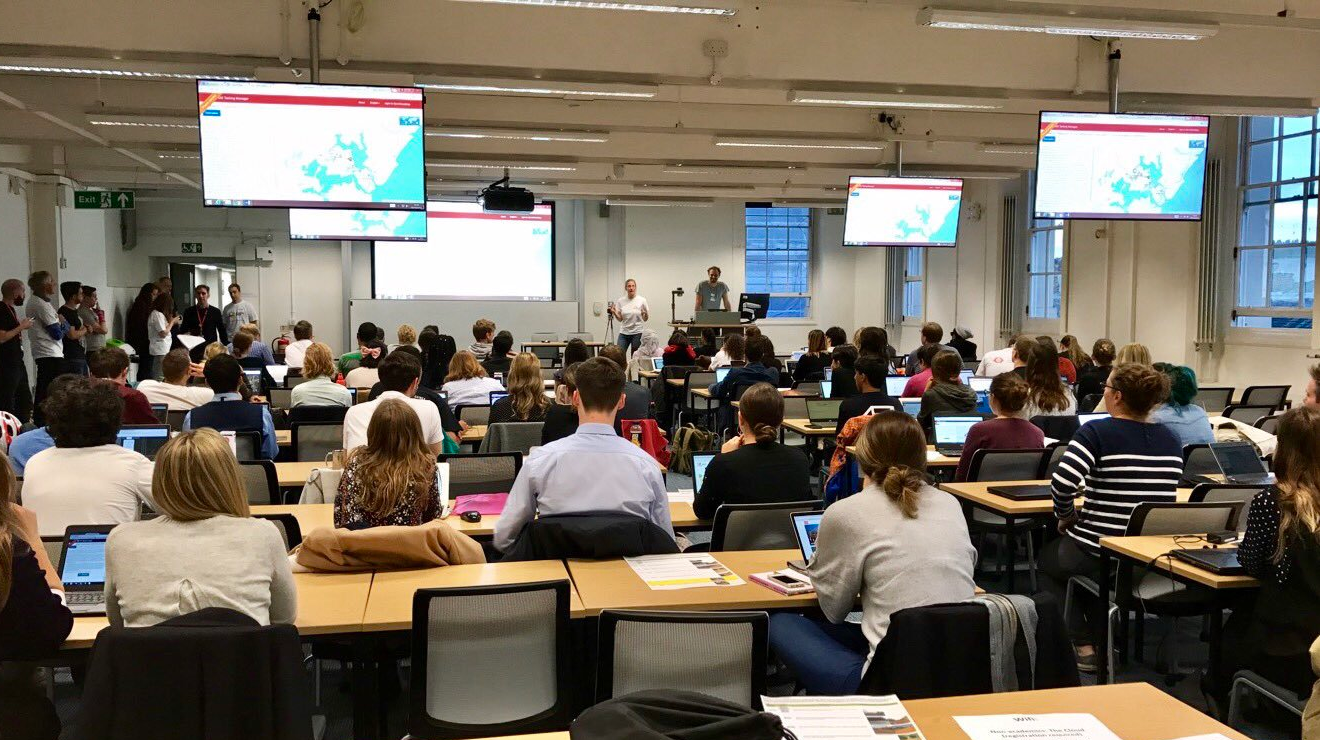
\includegraphics[width=0.7\textwidth]{images/MissingMapsMappingParty.png}
    \caption{A Missing Maps volunteer mapathon at King's College in London, UK, focusing on Malakal in South Sudan}
    \label{fig:Missing Maps Mapathon}
\end{figure}

The result of this example deployment would be a very high-resolution image of the entire camp complex in less than 10 days, for a total cost on the order of \$6,000 (4-5 flying days plus airfare and accommodation for two people from Tanzania). 

Furthermore, the imagery can be accompanied by substantial data; the digitization process automatically enables counts, and even sophisticated estimation procedures such as categorizing buildings by surface area (to assess what is likely a residence vs a school, religious facility, or other structure, making the estimates of people per structure much more accurate). 

Smaller camps would be cheaper, though the cost will not go down in a linear fashion as the expense of traveling to a site, obtaining permission to fly, sensitizing the authorities and population etc is required even for the smallest area. 

A number of African countries now host local drone operators under the umbrella of the Flying Labs, a sort of quasi-commercial franchise of WeRobotics, a Geneva-based humanitarian organization dedicated to the use of drone technology for good. The Flying Labs usually have some equipment and expertise in-country, which can reduce the cost of a deployment, particularly a small one. However, they function on a cost-recovery basis and often charge as much or more than similar commercial ventures; it's important not to assume that their price is the best that can be found.

There are several Ebees and other drones scattered through the MSF movement in various offices. A few informal trials have been done, but none have been conclusive or specifically focused on head counts. To our knowledge, no MSF section or office has stepped up to provide drone services to the movement, though the Innovation department of MSF-Japan has made some efforts in this direction (including the well-publicized work carrying TB samples to labs in Papua New Guinea). This probably makes sense; until the utility, security, and need for drone surveys is more clear, MSF should not invest in building internal capacity for drone use. However, pending more conclusive and systematic piloting of drone surveys (including for head counts) it may well become useful in the future for an internal MSF entity to acquire a full aerial surveying kit and expertise to provide to field missions at need. 

\subsubsection{Aircraft}
It's always been possible to take pictures out the window of an airplane or helicopter. We are aware of a few cases where this has been done in MSF projects (and in fact one of the authors of this report has previously leaned out the door of a UN helicopter to take pictures of a refugee camp for watsan planning purposes while on mission with MSF). However, for head counts, a simple snapshot doesn't provide sufficient resolution or context for population estimation (except for very small settlements, which are in any case easy to count).  

Since around 2016, there has been an explosion in development of of \textit{photogrammetry} software. This allows the analysis of photographs to align portions containing the same features, creating a composite image. 

\begin{figure}[H]
    \centering
    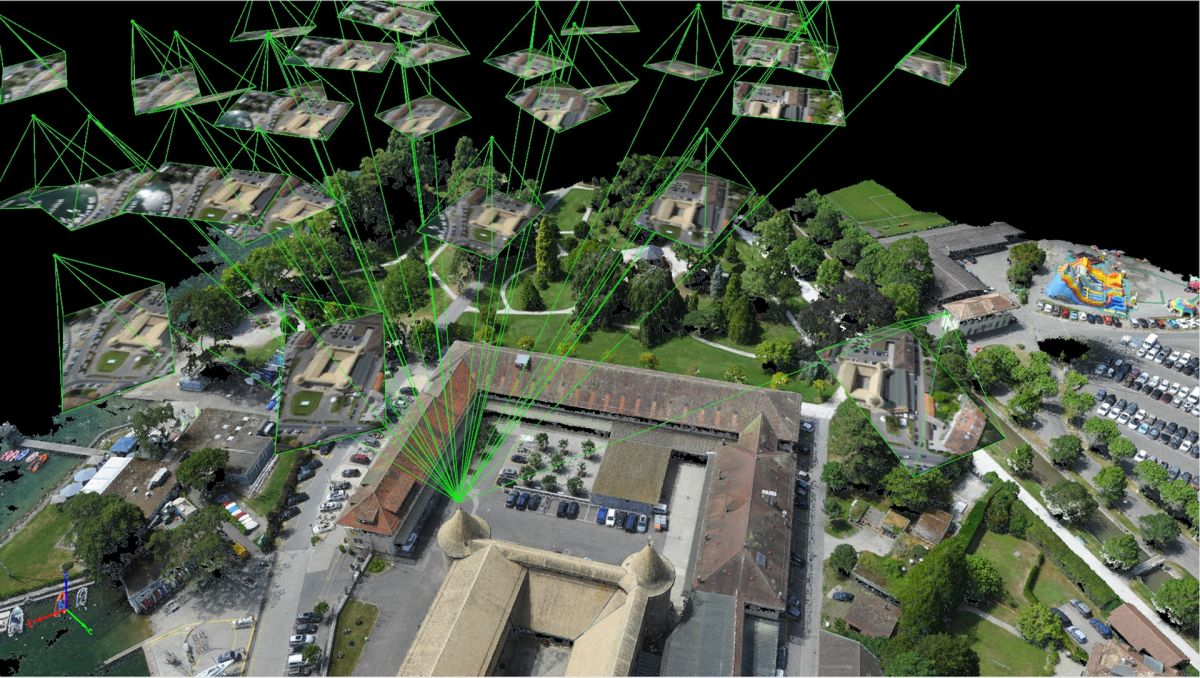
\includegraphics[width=0.7\textwidth]{images/rayCloud-pix4d-parallax-black.jpg}
    \caption{Photogrammetry can combine multiple photos into one image}
    \label{fig:Photogrammetry}
\end{figure}

Commercial software such as Pix4D, or open-source software such as OpenDroneMap (the authors' personal favorite) allow photographs taken from the air to be combined. 

MSF missions often have access to aircraft, whether it be small planes used to fly in and out of projects or UN helicopters in coordinated disaster responses. In many cases it's possible for minimal expense---or even free---to overfly a project area and take pictures. Small aircraft pilots will often allow MSF passengers to affix a camera to the outside of the plane (the classic GoPro-on-a-Cessna protocol).

\begin{figure}[H]
    \centering
    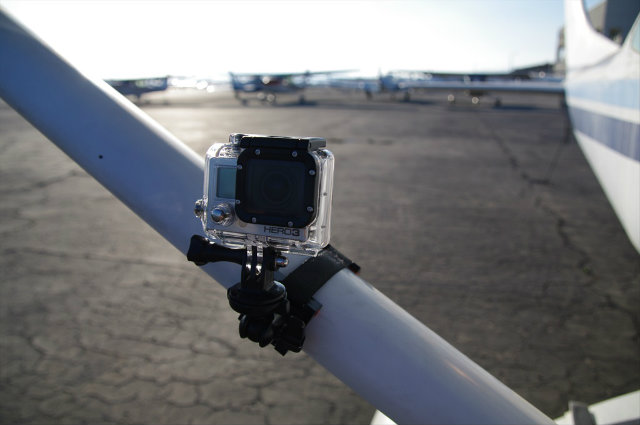
\includegraphics[width=0.45\textwidth]{images/GoPro_Cessna.jpg}
    \caption{A consumer GoPro camera affixed to the wing strut of a small Cessna}
    \label{fig:GoPro Cessna}
\end{figure}

Photographs taken in this fashion were, in previous years, mostly of novelty value. However, by running them through a photogrammetry package they can be made into seriously useful project assets capable of supporting frequent structure counts to estimate population and change.

\subsubsection{Kites and Balloons}
Where aircraft and drones are unavailable or sensitive, kites and balloons can provide a surprisingly robust method to gather aerial imagery. This would not be the best way to gather rapid imagery (it requires time, patience, and cooperative weather). It's not actually cheap; a proper kite or balloon mapping kit can easily cost as much as or more than a small drone such as a DJI Mavic Pro (around \$1,600), but once you have it you can use it cheaply for as long as you like.

In a setting where frequent image updates were desired, but the speed of acquisition was not overly critical, balloon or kite mapping might be a solution.

\begin{figure}[H]
\begin{subfigure}{0.5\textwidth}
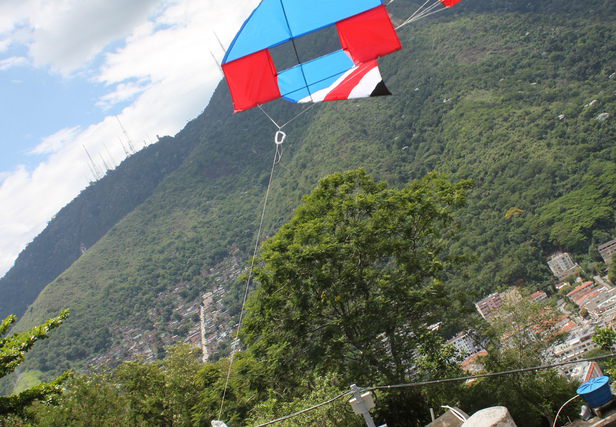
\includegraphics[width=0.9\linewidth, height=5cm]{images/Kite_mapping_in_Brazil.jpeg} 
\caption{Kite mapping in Brazil}
\label{fig:kite mapping}
\end{subfigure}
\begin{subfigure}{0.5\textwidth}
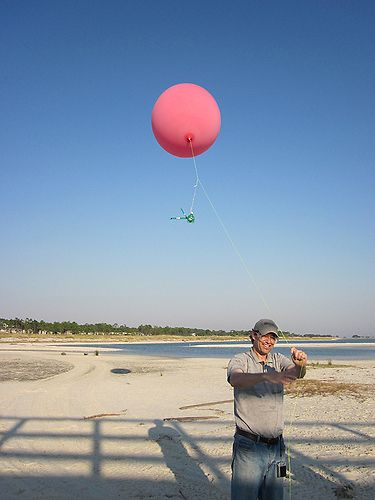
\includegraphics[width=0.9\linewidth]{images/Baloon_mapping.jpg}
\caption{Balloon mapping}
\label{fig:baloon mapping}
\end{subfigure}
\caption{Kite and balloon mapping can be less intimidating than drones)}
\label{fig:image2}
\end{figure}

Ultimately, balloons and kites are not likely to be a major component of a sensible Head Count toolkit; their use is limited to a narrow slice of contexts where aerial imagery is desired but drones or aircraft are impractical for some reason. However, they remain an option that could make the occasional project team quite happy.

\subsection{Mobile Data Collection}

\subsubsection{Community-Based Mobile Data Collection}
Mobile data collection is nothing new, however, in recent years it has become possible to use very low-educated people from within the beneficiary or local population, to gather data. 

\section{Recommendations}
MSF can take advantage of new opportunities. Not so much that there is new technology available---mobile data collection and drones have existed for some time now---but rather that both technologies have matured to the point that they can be used effectively in very low-resource settings.

\begin{itemize}
    \item MSF should consider using drones where rapid displacement has taken place in a setting that allows it without endangering the population or others (including MSF). Head counts are frequently dangerous and unpleasant exercises, and making use of newly available high-tech options---where ethical, appropriate and needed---is consistent with the duty of care to provide the best possible services to people.
    \item MSF should not consider mobile data collection to be the sole preserve of trained Community Health Care Workers or enumerators. Data collection can and should be seen as a collaboration and dialogue between the humanitarian community and the people we serve---use of local people, local devices, and open knowledge can greatly facilitate this. 
    
\end{itemize}

\section{Annex 1: Interviews}

\begin{center}
\begin{tabular}{|c|c|c|}  
 \hline
Country & Organization \\
\hline
CAR & \href{https://drive.google.com/open?id=1hKWbOf09AfBav2jGUfdhXv7ZLtpaG9QQRA_ePARLTn0}{MSF-OCBA} \\
\hline
Tanzania & Anonymous \\ 
\hline
Kenya & DRC \\
\hline
South Sudan	& MSF \\
\hline
Uganda & ICRC \\
\hline 
Uganda & UNHCR \\
\hline
Uganda & DRC \\
\hline
CAR & MSF \\
\hline
Somalia & MSF \\
\hline
Ethiopia & MSF OCBA \\
\hline
\end{tabular}
\end{center}

\end{document}
